%%%% fatec-article.tex, 2024/03/10

%% Classe de documento
\documentclass[
  a4paper,%% Tamanho de papel: a4paper, letterpaper (^), etc.
  12pt,%% Tamanho de fonte: 10pt (^), 11pt, 12pt, etc.
  english,%% Idioma secundário (penúltimo) (>)
  brazilian,%% Idioma primário (último) (>)
]{article}

%% Pacotes utilizados
\usepackage[]{fatec-article}
\Author{1}{Name={Muniz, Leandro Augusto de Souza\\ Albuquerque, Yan Gabriel de Olivira\\
Claudio, Diego Baltazar de Souza\\ Gomes, Igor Leite\\}}

\Author{2}{Name={\{ leandro.muniz@fatec.sp.gov.br \}\\ \{ yan.albuquerque@fatec.sp.gov.br \}\\ \{ diego.claudio@fatec.sp.gov.br \}\\ \{ igor.gomes4@fatec.sp.gov.br \}}}

%% Definição das palavras-chaves/keywords
\Keyword{1}{Freelancers}{Freelancers}
\Keyword{2}{Aplicativo}{Application}
\Keyword{3}{Geolocalização}{Geo-localization}

%%%% Resumo no idioma primário (brazilian)
\begin{Abstract}[brazilian]%% Idioma (brazilian ou english)
Este projeto aborda o tema da economia gig e suas relevâncias dentro mercado de trabalho atual, com foco principal em desenvolver a conexão entre contratantes e fornecedores de serviços que abrangem diversas areas de atuação, atualmente essa interação demanda de tempo e alta burocracia para ambas as partes envolvidas, prolongando o tempo de busca para solucionar essas demandas. A proposta visa utilizar geolocalização em tempo real e um sistema de avaliação dos serviços com base nas notas de avaliação.Essa abordagem facilita, agiliza e economiza tempo para atender as necessidades de contratantes e freelancers, aumentando a confiança e celeridade nos processos de interação de trabalhos rápidos. Os resultados preliminares indicam que o projeto possui o potencial de solucionar e promover conexões seguras e rápidas para serviços de freelancers.
\end{Abstract}

%%%% Resumo no idioma secundário (english)
\begin{Abstract}[english]%% Idioma (brazilian ou english)
This project addresses the topic of the gig economy and its relevance within the current job market, with the main focus on developing the connection between contractors and service providers that cover different areas of activity, currently this interaction demands time and high bureaucracy for both parties involved, prolonging the search time to resolve these demands. The proposal aims to use real-time geolocation and a service evaluation system based on evaluation scores. This approach facilitates, speeds up and saves time to meet the needs of contractors and freelancers, increasing confidence and speed in work interaction processes fast. Preliminary results indicate that the project has the potential to solve and promote secure and fast connections for freelance services.
\end{Abstract}

%% Processamento de entradas (itens) do índice remissivo (makeindex)
\makeindex%

%% Arquivo(s) de referências
\addbibresource{fatec-article.bib}

%% Início do documento
\begin{document}

% Seções e subseções
%\section{Título de Seção Primária}%

%\subsection{Título de Seção Secundária}%

%\subsubsection{Título de Seção Terciária}%

%\paragraph{Título de seção quaternária}%

%\subparagraph{Título de seção quinária}%

\section*{Introdução}%
\label{sect:intro}
No final de 2015, a Organização das Nações Unidas (ONU) desenvolveu a Agenda 2030, um plano de ação global contendo 17 metas destinadas a promoção da sustentabilidade, denominada Objetivos de Desenvolvimento Sustentável (ODS). Este trabalho está fortemente ligado ao alcance das metas apresentadas pela agenda abordando os seguintes tópicos: Promover o crescimento econômico inclusivo e sustentável, o emprego pleno e produtivo e o trabalho digno para todos, associado à ODS 8, que promove Trabalho decente e crescimento econômico. 

Nesse contexto, destaca-se a ascensão da gig economy, um termo que se refere ao modelo de trabalho caracterizado pela contração de serviços autônomos, com contratos flexíveis e de curta duração. Este modelo abrange uma variedade de profissões, como motoristas de aplicativos, entregadores, profissionais autônomos de serviços gerais e até trabalhadores especializados, como designers e programadores. A consolidação definitiva desse modelo teve início por volta de 1995, impulsionada pela evolução da internet e pelo surgimento de plataformas de contratação de serviços como CraigList, Elance, Odesk \cite{ROCKCONTENT2023} e posteriormente o desenvolvimento dos aplicativos Uber e Ifood.  

No Brasil, essa realidade é bastante evidente. No segundo trimestre de 2022, a taxa de informalidade atingiu 40\% \cite{IBGE2022}, esse percentual engloba profissionais vinculados à gig economy. Entre estes, destacam-se prestadores de serviços gerais, como pedreiros, pintores, encanadores, eletricistas, marceneiros e jardineiros. Esses trabalhadores enfrentam desafios significativos, como dificuldades para serem contratados, baixa visibilidade, carência de valorização profissional e ausência de garantias legais, o que contribui para um mercado mais vulnerável e carente de melhorias estruturais.  

Nesse sentido é importante destacar que a modalidade da economia gig tem sido objeto de debates, principalmente no que diz respeito aos interesses dos profissionais e das empresas intermediadoras. Conforme discutido por Rocha \cite{RochaFerreira2022}, o fenômeno de contratos flexíveis mediados por plataformas evidencia a necessidade de consolidação de proteções aos trabalhadores, apontando problemáticas como a falta de direitos trablhistas, remunerações desproporcionais e a utilização de algoritmos considerados não transparentes. 

Além do mais, sob a perspectiva dos contratantes, é possível observar ausências de garantias relacionadas à qualidade do serviço prestado, e, no caso específico de mulheres, destaca-se a questão de insegurança ao receberem profissionais desconhecidos em suas residências \cite{ESTADAO2020} 

Diante desse cenário evidencia-se a necessidade de mecanismo intermediadores que facilitem a contratação entre trabalhadores inseridos na gig economy e os contratantes, de forma transparente, segura e que valorize o trabalhador. Tais ferramentas podem contribuir para garantir maior segurança, formalidade e confiabilidade no processo, acabando por beneficiar ambas as partes. Além disso, tais mecanismos fomentam o crescimento econômico sustentável, visto que ampliam a divulgação e valorização dos profissionais e estabelecem uma uma padronização nas relações de prestação de serviço.  

Considerando essa demanda, este projeto propõe o desenvolvimento de uma plataforma web baseada na interação eficiente, na transparência e em critérios objetivos de qualidade e confiabilidade, voltada à divulgação e contratação de trabalhadores que prestam serviços sob demanda.  O modelo proposto vai além da simples intermediação de contratos, integrando mecanismos de verificação de competências e avaliações de qualidade dos serviços, o que aumenta a confiança entre as partes envolvidas. Assim, a proposta oferece uma solução que se adapta às exigências de um mercado de trabalho dinâmico e em constante evolução.

\section*{OBJETIVO} \label{sect:obj}

Atualmente, a principal forma de contratação relacionada a mão de obra especializada é realizada por meio de indicações ou anúncios, onde contratantes avaliam os candidatos com base em descrições e portfólios apresentados. No entanto, a seleção final geralmente é confirmada após conversas diretas ou pequenas tarefas iniciais para validar a adequação do profissional ao trabalho requerido, logo esse processo acaba levando um tempo maior para ser concluído, e muitas vezes existe a necessidade de uma solução mais ágil para solucionar tais demandas de serviço.\\

Este projeto visa como objetivo principal desenvolver uma aplicação para contratação de freelancers que seja eficiente e intuitiva, agregando aos profissionais autônomos uma ferramenta essêncial para divulgação de seu trabalho. Através desta aplicação, buscamos facilitar o processo de contratação de serviços especializados, permitindo que contratantes encontrem soluções adequadas para suas necessidades e que freelancers tenham acesso a uma ampla gama de oportunidades de trabalho. Para isso temos alguns outros objetivos a serem alcançados:


\subsection{Conexão e Dinâmica}
\subsubsection{Desenvolver uma aplicação que conecte contratantes e prestadores de serviços, facilitando a intermediação entre freelancers e empresas ou indivíduos que necessitam de serviços especializados. A plataforma será projetada para otimizar a busca e seleção de profissionais, oferecendo uma interface intuitiva e ferramentas de gestão que permitam aos usuários administrar suas contratações e projetos de maneira prática e organizada.}

\subsection{Pagamentos} 
\subsubsection{Criação de um ambiente seguro para a realização de transações financeiras diretamente pelo aplicativo, garantindo a segurança e eficiência entre contratantes e mão de obra qualificada. O sistema de pagamento integrado eliminará a necessidade de intermediários externos, oferecendo maior controle sobre o fluxo financeiro e assegurando a proteção dos dados dos usuários, com foco na transparência e na confiabilidade das operações.}

\subsection{Segurança e Confiabilidade}
\subsubsection{Proporcionar um ambiente seguro para a contratação de serviços, implementando mecanismos avançados de segurança como verificações de identidade, avaliações de usuários e medidas contra fraudes e abusos. Foco no desenvolvimento de uma plataforma confiável, onde tanto contratantes quanto freelancers possam realizar transações e acordos de trabalho com segurança e tranquilidade.}

\subsection{Ecossistema e Geolocalização} 
\subsubsection{Projetar a aplicação para fomentar um ecossistema de trabalho colaborativo e inclusivo, incentivando a diversidade entre profissionais de diferentes áreas e regiões geográficas. A plataforma terá recursos que facilitam a comunicação e a colaboração entre as partes, permitindo dessa maneira uma seleção mais eficaz dos profissionais localizados próximo ao local do contratante, poupando tempo para ambas as partes envolvidas e promovendo uma alta rotatividade de serviços locais.}


\section*{ESTADO DA ARTE} \label{sect:estadoarte}

É relevante observar que no contexto estado da arte, foram citados diversas aplicações e projetos que abrangem tópicos variados e soluções semelhantes à proposta neste trabalho, serão apresentados os aspectos mais relevantes de cada aplicação e suas funcionalidades relacionadas ao modelo de desenvolvimento para aplicações móveis e algumas arquiteturas utilizadas. Após a análise dos projetos existentes, observamos que todos têm como objetivo facilitar a conexão entre trabalhadores e consumidores, otimizando o processo de vendas e a contratação de profissionais. O nosso projeto se destaca ao incorporar a funcionalidade de geolocalização, permitindo a busca por prestadores de serviços freelancers mais próximos, o que aumenta a agilidade na resolução de demandas. Inicialmente, a aplicação é voltada para a contratação de serviços de manutenção e reparos; em versões futuras, planejamos expandir o escopo para incluir serviços adicionais, abrangendo áreas como tecnologia da informação e marketing digital, ampliando assim a gama de soluções oferecidas aos usuários.

\section{99FREELAS}
\subsubsection{A plataforma para contratação serviços de marketing digital \cite{99Freelas}, tornou-se um meio para as empresas se conectarem a freelancers que ofereçam serviços relacionados ao tema, trouxe como foco e diferencial meios de pagamento internos além da avaliação dos serviços por meio de classificação.}

\begin{figure}
\centering
\caption{99Freelas}
\label{fig:99Freelas}

\includegraphics[scale=0.5]{Illustrations/99Freelas.jpg}
\SourceOrNote{https://www.99freelas.com.br (2024)}
\end{figure}

\section{GETNINJAS}
\subsubsection{Esta ferramenta conhecida como \cite{GetNinjas} oferece um meio de solução para contratação de serviços freelancers para diversas finalidades: serviços domésticos, saúde, moda, beleza além da compra de diversos tipos de cursos, consultorias ou até mesmo aluguel de maquinários.}

\begin{figure}
\centering
\caption{GetNinjas}
\label{fig:GetNinjas}
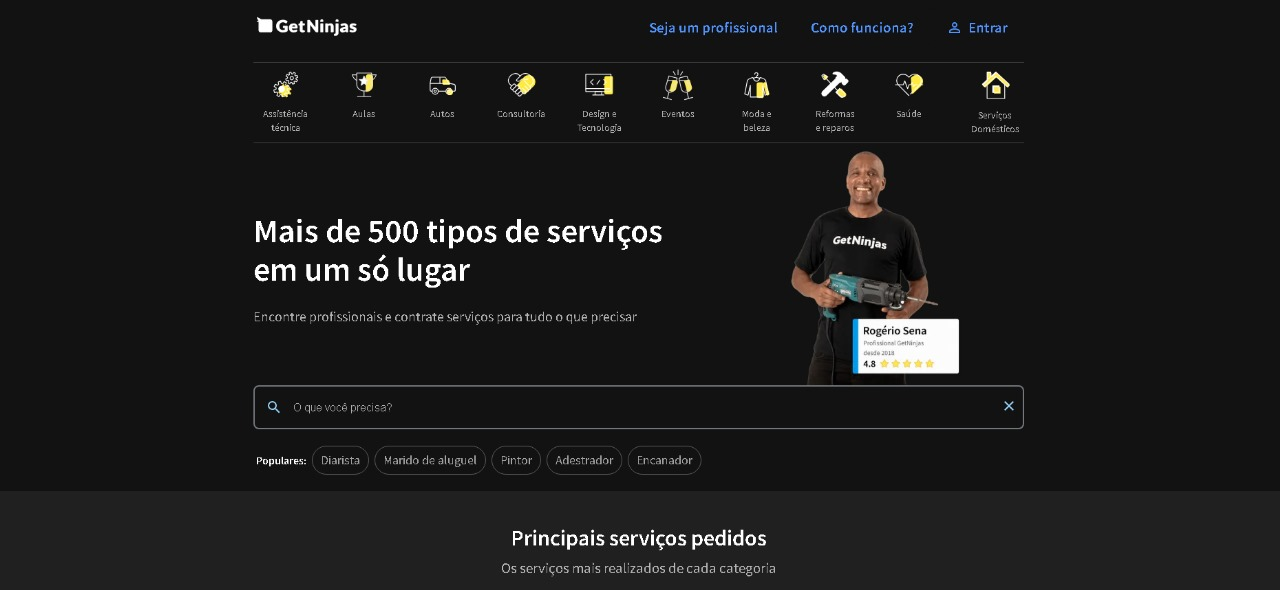
\includegraphics[scale=0.5]{Illustrations/GetNinjas.jpg}
\SourceOrNote{https://www.getninjas.com.br (2024)}
\end{figure}

\section{FIVERR}
\subsubsection{O \cite{Fiverr} é uma plataforma para intermediação de serviços relacionados a diversas áreas, como design gráfico, redação, marketing digital e programação permitindo que freelancers publiquem suas ofertas. A Fiverr conta com um sistema de avaliação que ajuda os usuários a escolher prestadores de serviços com base na reputação e na qualidade do trabalho, a plataforma também facilita a negociação e entrega de serviços, promovendo eficiência e transparência nas transações.}

\begin{figure}
\centering
\caption{Fiverr}
\label{fig:Fiverr}

\includegraphics[scale=0.5]{Illustrations/Fiverr.jpg}
% \SourceOrNote{https://www.fiverr.com/?source=top_nav (2024)} % O vscode não tá aceitando adicionar essa fonte aqui
\end{figure}

\section{API PARA CONTRATAÇÃO DE SERVIÇOS DE INFORMÁTICA}
\subsubsection{Este estudo \cite{Silva2022} trata-se sobre uma aplicação para contratação de serviços de informática, com o intuito de ajudar iniciantes da área, por conta do tempo de experiência exigido pelos contratantes, é um auxilio para alavancar profissionais que estão ingressando no ramo tecnológico.}

\section{UTILIZAÇÃO DE API PARA GEOLOCALIZAÇÃO EM TEMPO REAL DE ENCOMENDAS PEDIDAS POR MEIO DE UM APLICATIVO MOBILE MULTIPLATAFORMA}
\subsubsection{Este projeto \cite{Oliveira2022} é uma proposta de e-commerce com serviço de geolocalização para publicação, seleção, envio e rastreio de encomendas que conecta motoristas, remetentes e destinatários para maior facilidade e agilidade da entrega.}

\begin{figure}
\centering
\caption{Utilização de api para geolocalização em tempo real de encomendas pedidas por meio de um aplicativo mobile multiplataforma}
\label{fig:Oliveira12022}
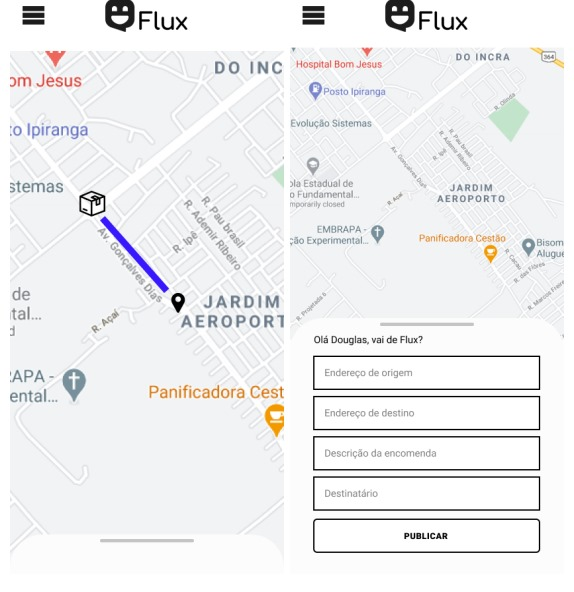
\includegraphics[scale=0.8]{Illustrations/Oliveira12002.jpg}
\SourceOrNote{https://repositorio.utfpr.edu.br/jspui/handle/1/32355(2024)}
\end{figure}

\section*{METODOLOGIA} \label{sect:metodologia}

\section{Planejamento}
\subsection{Do Planejamento}
\subsubsection{A metodologia deste projeto seguiu um fluxo estruturado que compreende as etapas de planejamento, prototipação e desenvolvimento. Durante o planejamento foram definidas as principais características do sistema, englobando serviços, interatividade, interface e identidade visual, aspectos essenciais para a fase de prototipação onde foram utilizados softwares como Figma para o design visual e brModelo para modelagem de banco de dados conceitual.}

\section{Prototipação}
\subsection{Identidade Visual e Protótipo }
\subsubsection{Por meio do software Figma, foi desenvolvida a identidade visual e o design do sistema, criando um protótipo de alta fidelidade, o protótipo inclui telas essenciais, como Tela Principal, Tela de Usuário, Tela de Chamado e Menu, garantindo a representação das funcionalidades principais. A navegação entre as telas foi projetada para ser intuitiva e funcional, possibilitando ao usuário uma experiência de uso fluida e facilitando a validação das interações do sistema}

\subsection{Banco de dados }
\subsubsection{A utilização da ferramenta brModelo possibilitou a criação de um modelo conceitual de banco de dados para o sistema, facilitando a estruturação lógica dos dados e suas relações. Embora o modelo ainda esteja em fase conceitual, ele oferece uma visão clara das entidades e dos relacionamentos necessários para o funcionamento do sistema, permitindo o planejamento detalhado dos requisitos de dados que serão implementados na fase de desenvolvimento.}

\subsection{Landing Page}
\subsubsection{Embora o foco do nosso sistema seja a aplicação móvel, também foi desenvolvida uma página web utilizando HTML, CSS e Bootstrap. Esta página tem como objetivo fornecer informações detalhadas sobre os serviços oferecidos, apresentando as funcionalidades disponíveis e orientando os usuários sobre as diversas possibilidades de uso. Além disso, a página inclui um atalho direto para o download do aplicativo, otimizando a acessibilidade e facilitando a interação dos usuários com a plataforma.}

\subsection{Home Page }
\subsubsection{Também foi desenvolvida uma Home page em Node.js com o framework Express para ampliar a acessibilidade e promover informações sobre o serviço, essa página web funciona como uma interface informativa, utilizando o Express para gerenciar requisições HTTP e garantindo respostas rápidas e estruturadas aos usuários. A integração é feita por meio de um banco de dados MySQL que fornece consulta e exibição dinâmica de informações, como listagem de serviços e perfis de freelancers diretamente na página, por meio dessa arquitetura facilita futuras expansões, como a implementação de formulários de contato que armazenam dados no MySQL, além de outras funcionalidades de interação direta entre o frontend e o backend, permitindo um gerenciamento eficiente de dados em tempo real.} 

\begin{itemize}
\item \textbf{bcrypt}: Foi utilizada para gerenciar a criptografia de senhas, garantindo a segurança no armazenamento de credenciais, por meio de hashing.
\item \textbf{ejs}: Serviu como motor de templates, permitindo a renderização dinâmica de páginas HTML com dados enviados pelo servidor, facilitando a interação entre front-end e back-end.
\item \textbf{express}: Atendeu como o framework principal para a criação do servidor, fornecendo uma estrutura simplificada para gerenciar rotas, requisições e respostas HTTP.
\item \textbf{express-flash}: Foi usada para exibir mensagens de feedback temporárias (flash messages), como notificações de sucesso ou erro, entre requisições do usuário.
\item \textbf{express-session}: Gerenciou sessões de usuário no servidor, armazenando dados temporários e garantindo persistência entre requisições enquanto o usuário estivesse autenticado.
\item \textbf{mysql2}: Proporcionou uma interface otimizada para conexão e execução de operações no banco de dados MySQL, com suporte a promessas para simplificar o código assíncrono.
\item \textbf{nodemon}: Facilitou o desenvolvimento ao reiniciar automaticamente o servidor toda vez que alterações no código foram detectadas, aumentando a produtividade.
\item \textbf{sequelize}: Foi empregada como um ORM (Object-Relational Mapping), permitindo manipulação de dados no banco de forma programática, abstrata e eficiente, ao mapear tabelas para modelos em JavaScript.
\end{itemize}

\subsection{Algoritmo Merge Sort}

O algoritmo \texttt{Merge Sort} foi implementado pois futuramente com uma grande introdução de dados na Aplicação, surgirá a necessidade dessa ordenação que utiliza o princípio de \textit{dividir e conquistar}, que consiste em dividir o array em subarrays menores, ordenando esses subarrays e, em seguida, os combina (ou \textit{merge}) para obter a lista ordenada. Abaixo está a explicação do algoritmo implementado no código:

\begin{itemize}
\item \textbf{Função mergeSort}: Recebe um array \texttt{arr} e uma chave \texttt{key} como parâmetros e realiza a ordenação.
\begin{itemize}
\item Caso o array tenha 0 ou 1 elemento, ele já está ordenado e é retornado imediatamente.
\item Caso contrário, o array é dividido em duas metades:
\begin{itemize}
\item \texttt{left}: A primeira metade do array.
\item \texttt{right}: A segunda metade do array.
\end{itemize}
 \item Essas duas metades são ordenadas recursivamente, utilizando chamadas recursivas da função \texttt{mergeSort}.
\item Após as chamadas recursivas, as duas metades ordenadas são combinadas por meio da função \texttt{merge}.
\end{itemize}
    
\item \textbf{Função merge}: Realiza a mesclagem das duas metades ordenadas.
\begin{itemize}
\item Inicializa um array vazio \texttt{result}, que armazenará os elementos ordenados.
\item Utiliza dois índices, \texttt{i} e \texttt{j}, para percorrer as metades \texttt{left} e \texttt{right}, respectivamente.
\item A comparação entre os elementos das duas metades é feita com base na chave \texttt{key}.
\item Caso o valor da chave seja \texttt{"Não Classificado"}, ele é colocado no final da ordenação.
\item Caso contrário, o valor é comparado de forma decrescente e o menor valor é inserido primeiro no array \texttt{result}.
\item Após a comparação, o índice é incrementado para a próxima posição na respectiva metade.
\item Quando todos os elementos de uma das metades forem processados, o restante da outra metade é concatenado ao array \texttt{result}.
\end{itemize}
    
\item \textbf{Retorno da função mergeSort}: O array ordenado é retornado pela função \texttt{mergeSort}.
\end{itemize}

\subsection{Banco de Dados}
\subsubsection{O banco de dados foi criado no \textbf{MySQL Workbench} com o nome de \textit{AppBeelancer}, e o ambiente de desenvolvimento foi configurado utilizando o \textbf{XAMPP} para fornecer a infraestrutura necessária, incluindo o servidor Apache e o MySQL para a criação e gerenciamento do banco de dados. A database \textit{AppBeelancer} consistiu em oito tabelas principais:}

\begin{itemize}
\item \textbf{Usuarios}: Armazenou informações dos usuários do sistema, como dados de autenticação e perfil.
\item \textbf{Enderecos}: Continha os endereços de usuários, freelancers e clientes, incluindo detalhes como rua, cidade, estado e código postal.
\item \textbf{Freelancers}: Registrou os dados dos freelancers, como nome, especialização e status.
\item \textbf{Especialidades}: Armazenou as habilidades ou especializações oferecidas pelos freelancers.
\item \textbf{Telefones}: Guardou os números de telefone, associando-os a usuários ou freelancers, com informações sobre o tipo e formato do número.
\item \textbf{Clientes}: Registrou informações sobre os clientes que contrataram os serviços dos freelancers, incluindo os campos \texttt{createAt} e \texttt{updateAt} para rastrear as datas de criação e atualização dos registros.
 \item \textbf{EspxFrees}: Foi responsável pela associação entre freelancers e especialidades, recebendo as chaves estrangeiras de ambas as tabelas.
\item \textbf{Chamados}: Registrou os serviços requisitados pelos clientes, incluindo detalhes sobre o tipo de serviço, status e histórico.
\end{itemize}

\section*{RESULTADOS PRELIMINARES}\label{sect:resultados}

% O propósito da seção de resultados, como o próprio nome indica, é revelar o que foi encontrado na pesquisa. Essa parte do artigo estará composta dos dados relevantes obtidos e sintetizados pelo autor. 

% Nesta seção, você deverá apresentar todos os elementos solicitados no mapa mental relacionados ao seu projeto: diagramas, protótipos, modelo de negócios, principais funções e componentes desenvolvidos. Para tanto, na subseção a seguir, você poderá consultar como é feita a inserção de figuras, fluxogramas, fotografias, gráficos, tabelas e quadros.

% \subsection*{Ilustração e Tabela}

% Independentemente da ilustração (figura, fluxograma, fotografia, gráfico, quadro, entre outras) ou tabela inserida no trabalho, sua identificação deve aparecer na parte superior. Esta identificação deve ser precedida da palavra designativa, seguida de seu número de ordem de ocorrência no texto, em algarismos arábicos, travessão e do respectivo título.

% Após a ilustração ou tabela, na parte inferior, indicar a fonte consultada (mesmo sendo produção do próprio autor), legenda, notas e outras informações necessárias à sua compreensão (se houver). A ilustração deve ser citada no texto e inserida o mais próximo possível do trecho a que se refere. A seguir, encontra-se um exemplo para a inserção de um elemento do tipo Gráfico, o \Cref{grph:example}.

% \begin{graph}[!h]
% \centering
% \SetCaptionWidth{\ifbool{@LayoutA}{0.7}{0.72}\linewidth}
% \caption{Exemplo de gráfico}%
% \label{grph:example}
% 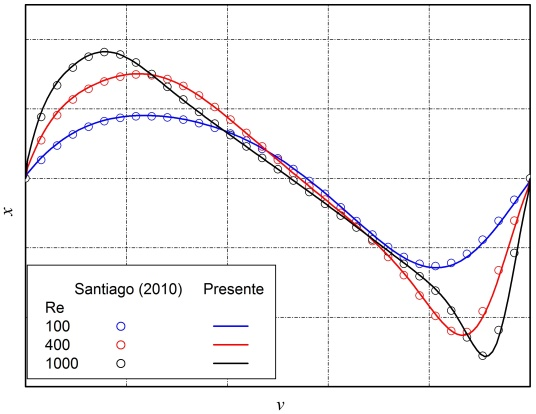
\includegraphics[width = \CaptionWidth]{grph-example}
% \SourceOrNote{Autoria Própria (2024)}
% \end{graph}

% Em computação, é muito comum a utilização de fluxogramas, para documentar, estudar, planejar, melhorar e comunicar processos complexos por meio de diagramas claros e fáceis de entender. Um fluxograma é um diagrama que descreve um processo, sistema ou algoritmo de computador. O \Cref{fcht:ex-algorithm} é um dos vários exemplos deste tipo de ilustração que pode ser gerado ou editado na ferramenta \textit{online} \href{http://www.lucidchart.com/}{Lucidchart}, entre outras.

% \begin{flowchart}[!htb]
% \centering
% \caption{Exemplo de fluxograma de algoritmo}%
% \label{fcht:ex-algorithm}
% 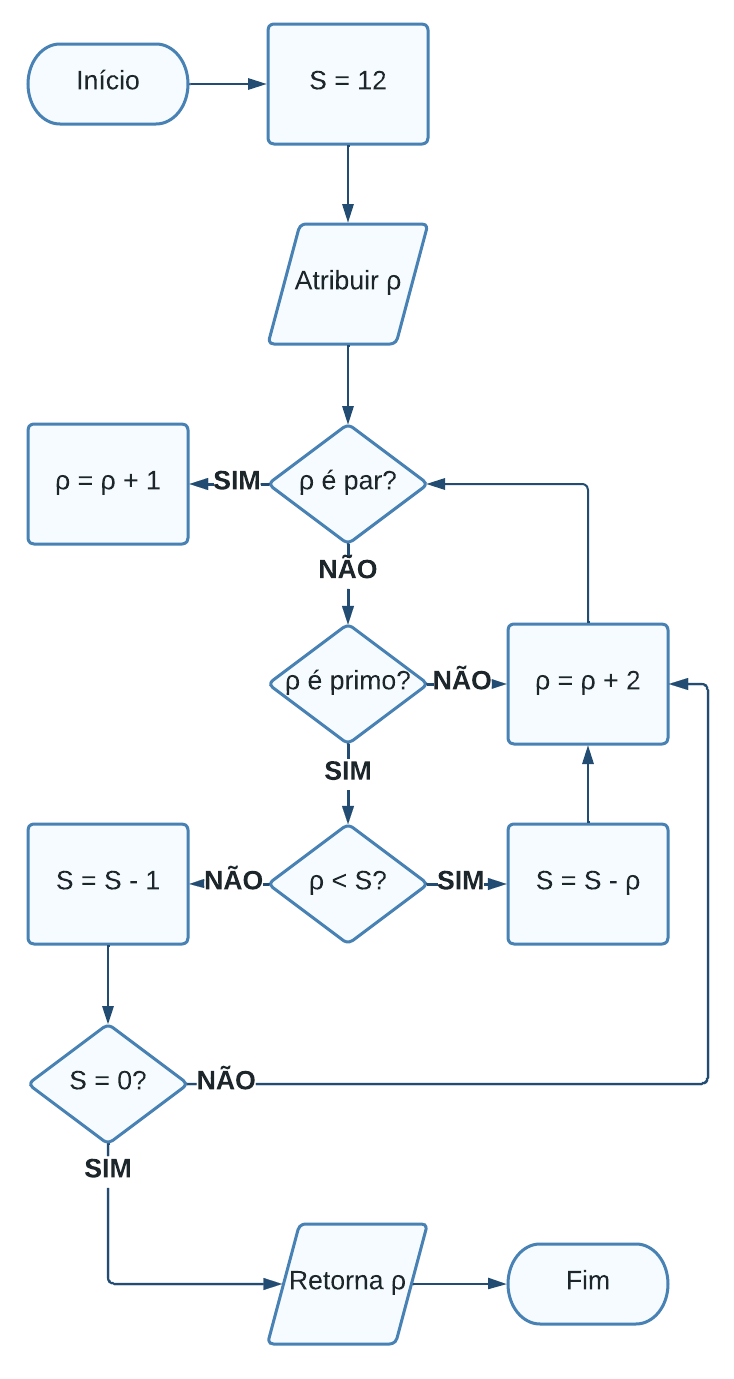
\includegraphics[scale=0.4]{fcht-ex-algorithm}
% \SourceOrNote{Autoria Própria (2024)}
% \end{flowchart}

% O LaTeX tem uma biblioteca específica para utilizar imagens no documento. O pacote graphicx habilita um ambiente chamado figure, que permite que você insira imagens de uma forma simples no texto. A \Cref{fig:example-image-duck} é um exemplo deste tipo de ilustração.

% \begin{figure}[!h]
% \centering
% \caption{Exemplo de figura}%
% \label{fig:example-image-duck}
% \includegraphics[scale=1.2]{example-image-duck}
% \SourceOrNote{Autoria Própria (2024)}
% \end{figure}

% Caso seja necessário, você ainda poderá inserir fotografias, por meio do ambiente \textit{photograph}, conforme ilustrado na \Cref{phot:pg-campus}.

% \begin{photograph}[!h]
% \centering
% \SetCaptionWidth{\ifbool{@LayoutA}{0.7}{0.72}\linewidth}
% \caption{Fachada da Fatec de Registro}%
% \label{phot:pg-campus}
% \savebox0{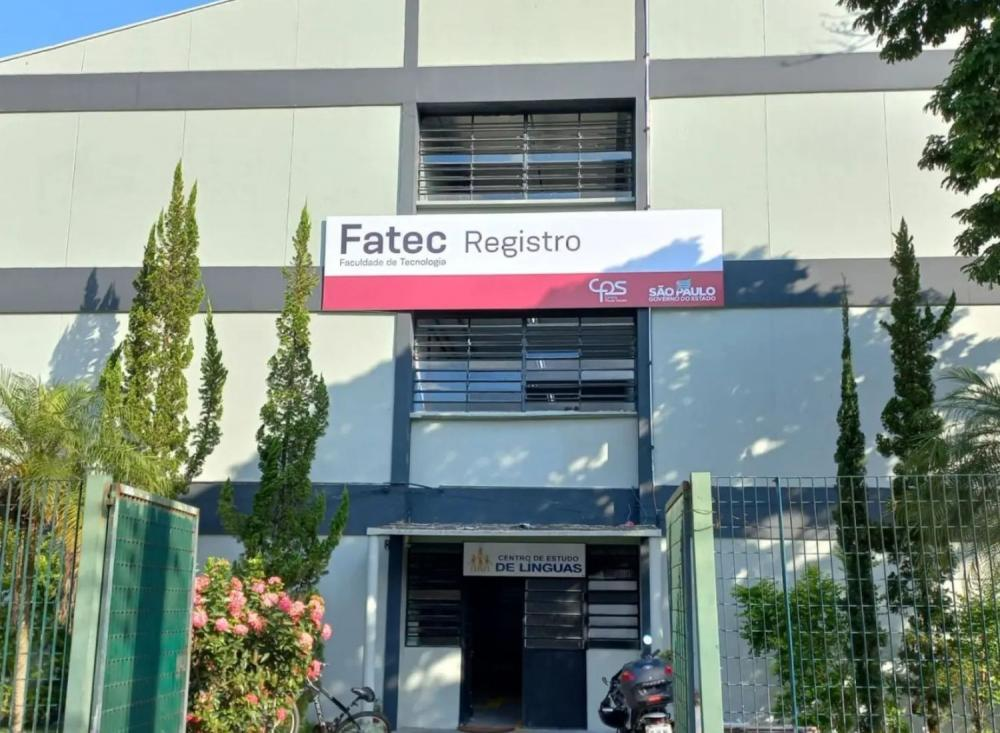
\includegraphics[width = \CaptionWidth]{Illustrations/fachada-fatec.jpg}}
% \usebox0%
% \SourceOrNote{Autoria Própria (2024)}
% \end{photograph}

% Outro elemento visual bastante utilizado na seção de Resultados são as tabelas, pois elas fornecem uma estrutura visualmente organizada para apresentar dados, tornando a leitura e a compreensão do conteúdo mais fácil para o leitor. As células, linhas e colunas ajudam a alinhar informações de maneira sistemática.

% Para conjuntos de dados comparativos, as tabelas são particularmente úteis. Elas possibilitam a disposição lado a lado de informações relacionadas, facilitando a comparação direta entre diferentes elementos.

% Tabelas e quadros devem estar centralizados e conter apenas dados imprescindíveis, evitando-se que sejam muito extensos, não repetindo dados já inseridos no texto, ou vice-versa. O formato de tabela pode ser observado na \Cref{tab:example}.

% \begin{table}[!htb]
% \centering
% \SetCaptionWidth{0.5\linewidth}
% \caption{Exemplo de tabela}%
% \label{tab:example}
% \begin{tabularx}{\CaptionWidth}{@{}XY@{}}
% \toprule%
% \rowcolor{TableColor}
% \multicolumn{1}{Y}{\textcolor{white}{Idade}}           &
% \multicolumn{1}{Y}{\textcolor{white}{Percentual (\%)}} \\
% \midrule%
% Até 20 anos     & 0  \\
% De 21 a 30 anos & 10 \\
% De 31 a 40 anos & 20 \\
% De 41 a 50 anos & 30 \\
% \bottomrule%
% \end{tabularx}
% \SourceOrNote{Adaptada de \textcite{Beltrano2021}}
% \end{table}

% No caso de quadros, deve ser seguida a estrutura demonstrada no \Cref{tfrm:typography}.
% Caso os dados sejam inéditos e provenientes de uma pesquisa realizada pelos próprios autores do trabalho, essa especificação deve constar na fonte com o ano da pesquisa de campo.
% Nesse caso, a fonte deve ser: Autoria Própria (2024).

% \begin{tabframed}[!htb]
% \centering
% \caption{Tipografia das seções}%
% \label{tfrm:typography}
% \begin{tabularx}{\linewidth}{?{}p{20mm}|X|p{45mm}?{}}%% CHKTEX 44
% \toprule%
% \rowcolor{TableColor}
% \multicolumn{1}{?{}c|}{\textcolor{white}{Seção}}   &
% \multicolumn{1}{c|}{\textcolor{white}{Tipografia}} &
% \multicolumn{1}{c?{}}{\textcolor{white}{Exemplo}}  \\
% \midrule%
% Primária                     &
% Letras maiúsculas em negrito &
% \textbf{1 SEÇÃO PRIMÁRIA}    \\
% \midrule%
% Secundária                    &
% Letras maiúsculas sem negrito &
% 1.1 SEÇÃO SECUNDÁRIA          \\
% \midrule%
% Terciária                                                             &
% Letra inicial de todas as palavras em maiúscula, sem negrito &
% 1.1.1 Seção Terciária                                                 \\
% \midrule%
% Quaternária                                                          &
% Letra inicial da primeira palavra em maiúscula, sem negrito &
% 1.1.1.1 Seção quaternária                                            \\
% \midrule%
% Quinária                                                                          &
% Letra inicial da primeira palavra em maiúscula, sem negrito e em itálico &
% \textit{1.1.1.1.1 Seção quinária}                                                 \\
% \bottomrule%
% \end{tabularx}
% \SourceOrNote{Autoria Própria (2024)}
% \end{tabframed}

% Quadros e tabelas podem ser inseridos neste documento usando os ambientes \texttt{tabframed} e \texttt{table}, respectivamente, conforme exemplos no arquivo-fonte deste modelo. A geração ou edição desses elementos visuais pode ser realizada por meio de ferramentas \textit{online}, tais como: \href{http://www.tablesgenerator.com/}{Tables Generator} e \href{http://www.latex-tables.com/}{Latex Tables Editor}, entre outras.

% \subsection*{Equações}

% Equações podem ser inseridas neste documento usando o ambiente  \texttt{equation}, como ilustrado na \Cref{eq:u}.

% \begin{equation}%
% \label{eq:u}
% u = \beta \operatorname{sen} \left(\pi x\right) \frac{\left(e^{2x} - 1\right) \left(e^y - 1\right)}{\left(e^2 - 1\right) \left(e - 1\right)}
% \end{equation}

% Símbolos matemáticos (ou equações mais simples) podem ser inseridos ao longo do texto de um parágrafo usando o ambiente do Latex \texttt{math}. É possível ainda, a utilização de ferramentas onlines para a geração ou edição de equações, tais como: \href{http://formulasheet.com/}{Formula Sheet} e \href{http://www.tutorialspoint.com/latex_equation_editor.htm}{Latex Equation Editor}.



\section*{CONCLUSÃO}\label{sect:conclusao}

% Apresente aqui as conclusões do seu trabalho, verifique se o objetivo foi cumprido, apresenta respostas para o problema da pesquisa, relate as limitações e as recomendações do estudo. Por fim, coloque sugestões para trabalhos futuros.

\printbibliography

%% Elementos pós-textuais (opcionais): Apêndice e Anexo
%Caso for utilizar, basta retirar o símbolo de % na frente do comando
%%%%% Elementos pós-textuais
%%
%% Glossário, apêndices, anexos e índice remissivo (opcionais).

%% Apêndices
\begin{Appendix}

\section{Título de Apêndice}%
\label{sect:apx-a1}

Exemplo de apêndice (\Cref{sect:apx-a1}) em uma seção de \nameref{sect:appendix}.

\subsection{Título de Seção Secundária de Apêndice}%
\label{ssect:apx-a2}

Exemplo de seção secundária de apêndice (\Cref{ssect:apx-a2}).

\subsubsection{Título de Seção Terciária de Apêndice}%
\label{sssect:apx-a3}

Exemplo de seção terciária de apêndice (\Cref{sssect:apx-a3}).

\paragraph{Título de seção quaternária de Apêndice}%
\label{prgh:apx-a4}

Exemplo de seção quaternária de apêndice (\Cref{prgh:apx-a4}).

\subparagraph{Título de seção quinária de Apêndice}%
\label{sprgh:apx-a5}

Exemplo de seção quinária de apêndice (\Cref{sprgh:apx-a5}).

\end{Appendix}

%% Anexos
\begin{Annex}

\section{Título de Anexo}%
\label{sect:anx-a1}

Exemplo de anexo (\Cref{sect:anx-a1}) em uma seção de \nameref{sect:annex}.

\subsection{Título de Seção Secundária de Anexo}%
\label{ssect:anx-a2}

Exemplo de seção secundária de anexo (\Cref{ssect:anx-a2}).

\subsubsection{Título de Seção Terciária de Anexo}%
\label{sssect:anx-a3}

Exemplo de seção terciária de anexo (\Cref{sssect:anx-a3}).

\paragraph{Título de seção quaternária de Anexo}%
\label{prgh:anx-a4}

Exemplo de seção quaternária de anexo (\Cref{prgh:anx-a4}).

\subparagraph{Título de seção quinária de Anexo}%
\label{sprgh:anx-a5}

Exemplo de seção quinária de anexo (\Cref{sprgh:anx-a5}).

\end{Annex}

%% Índice remissivo
\printindex%


%% Fim do documento
\end{document}